\subsection{Lab3:Grid position de WX GUI}
%*********************
\begin{frame}{}

\pgfdeclareimage[width=\paperwidth,height=\paperheight]{bg}{imagenes/fondo_lab}
\setbeamertemplate{background}{\pgfuseimage{bg}}

\bfseries{\textrm{\LARGE Lab3\\ \LARGE Grid position de \newline WX GUI}}
\raggedright
\end{frame}
%*********************

\begin{frame}{Grid position}

\pgfdeclareimage[width=\paperwidth,height=\paperheight]{bg}{imagenes/fondo3}
\setbeamertemplate{background}{\pgfuseimage{bg}}

\textbf {Posicionamiento de rejilla} \\
\vspace{2mm}
GRC ofrece varios receptores gráficos y controles gráficos para crear gráficos de flujo wx-gui.(scope sink, fft sink, number sink, waterfall sink, constellation sink, slider control, and chooser control) Cada uno de estos elementos gráficos tiene un parámetro de posición de cuadrícula para un posicionamiento preciso.

\end{frame}
%-----------------------------------

\begin{frame}{Grid position}

\begin{figure}[H]
\centering
\vspace{-3mm}
\includegraphics[width=0.9\textwidth]{parte1/lab3/pdf/lab0_1.pdf}


\end{figure}

\end{frame}
%-----------------------------------

\begin{frame}{Grid position}

El tramo de fila especifica el número de filas hacia abajo desde la posición de la fila, y el tramo de columna especifica el número de columnas a la derecha de la posición de la columna. Por lo tanto, el tramo debe ser al menos (1, 1) para ocupar el mínimo de 1 celda de cuadrícula.

\end{frame}
%-----------------------------------

\begin{frame}{Grid position}

\begin{figure}[H]
\centering
\vspace{-3mm}
\includegraphics[width=0.9\textwidth]{parte1/lab3/pdf/lab0_2.pdf}
\end{figure}

\end{frame}
%-----------------------------------

\begin{frame}{Grid position}

\begin{figure}[H]
\centering
\vspace{-3mm}
\includegraphics[width=0.9\textwidth]{parte1/lab3/pdf/lab0_3.pdf}
\end{figure}

\end{frame}
%-----------------------------------

\begin{frame}{Grid position}

Se realizará un ejemplo con una señal tipo guassiana donde se mostrara, con diferentes lugares de posiciones en las cuales se podrá variar la frecuencia y la señal de ruido con un text box en el cual se ingresará los valores que se desean para el fft, y un static text donde mostrará la amplitud de la señal que estará fija, y como resultado tendemos una gráfica de una señal en el dominio de la frecuencia la cual será FFT.

\end{frame}
%-----------------------------------

\begin{frame}{Señal FFT con Grid position}

\begin{figure}[H]
\centering
\vspace{-3mm}
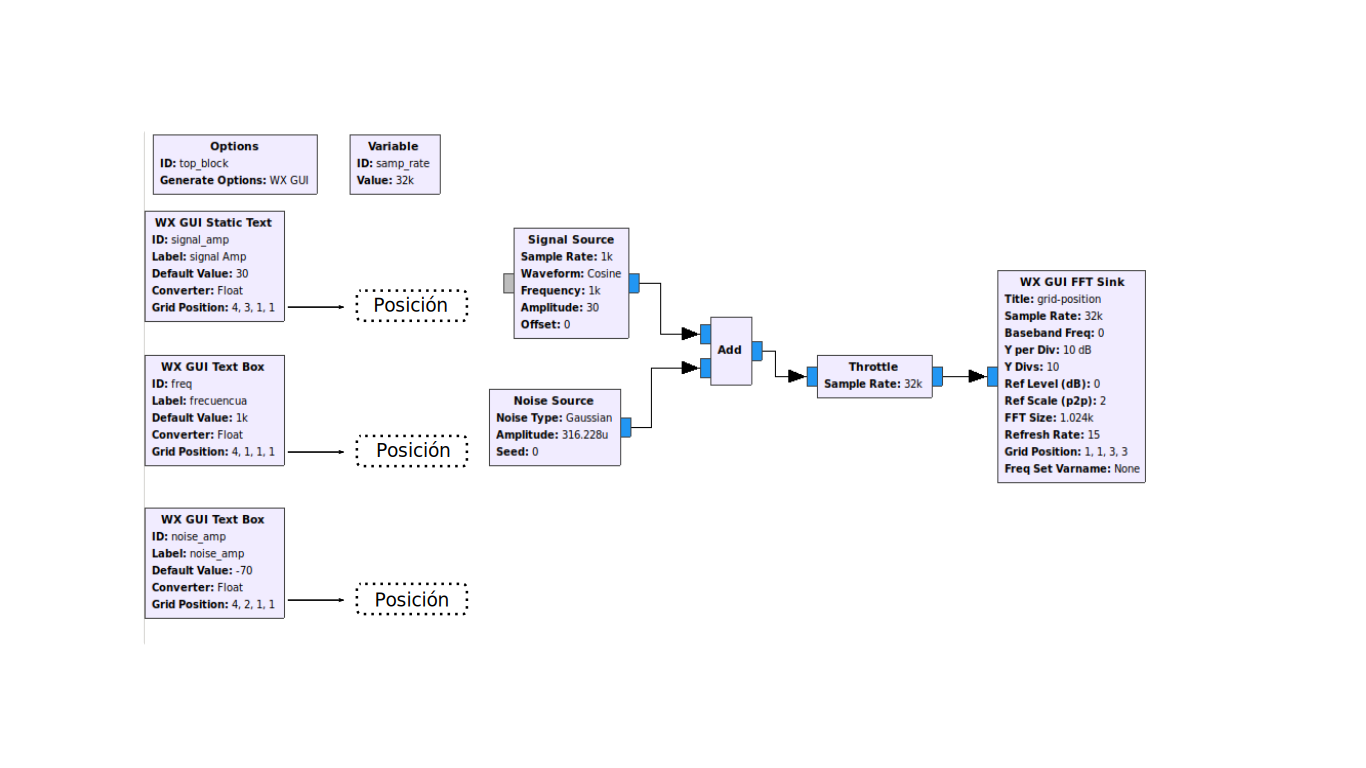
\includegraphics[width=0.9\textwidth]{parte1/lab3/pdf/lab0_4.pdf}
\end{figure}

\end{frame}
%-----------------------------------
\begin{frame}{Señal FFT con Grid position}

\begin{figure}[H]
\centering
\vspace{-3mm}
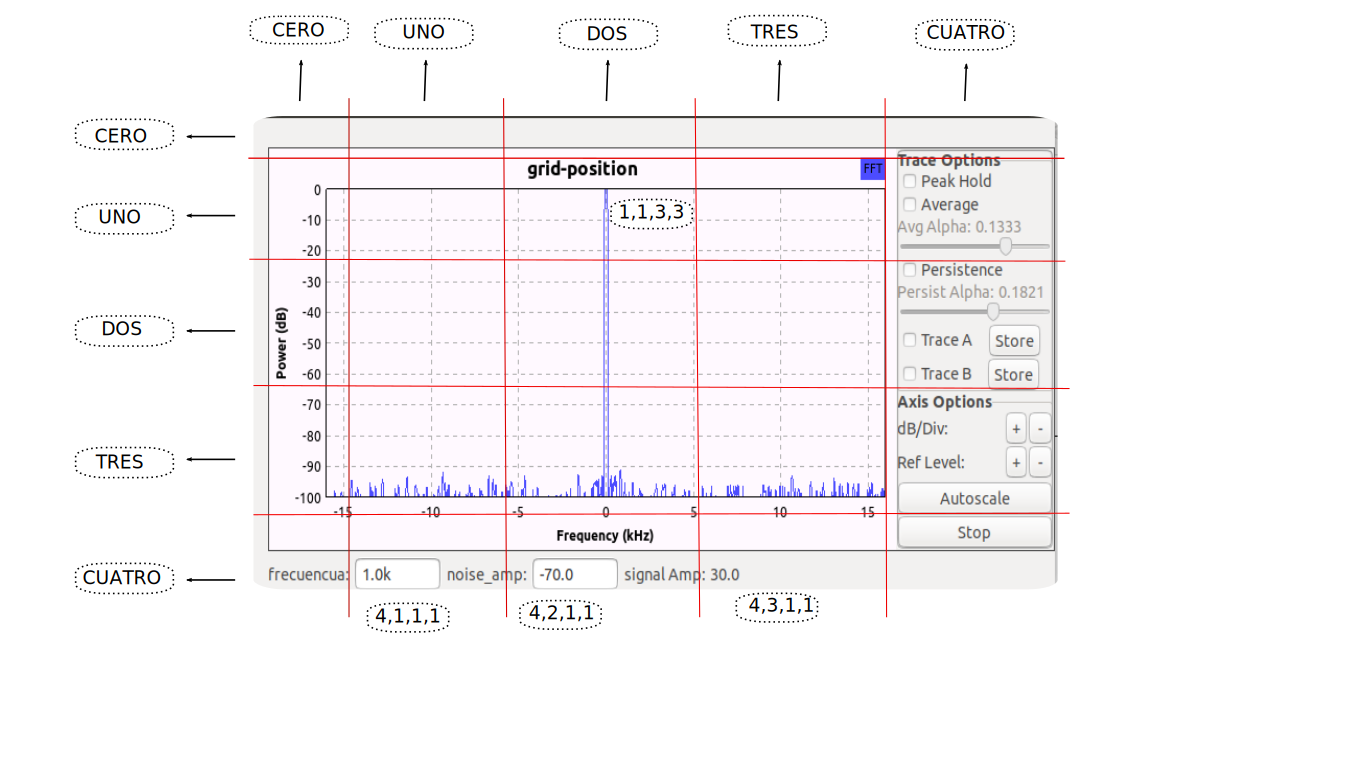
\includegraphics[width=0.9\textwidth]{parte1/lab3/pdf/lab0_5.pdf}
\end{figure}

\end{frame}
%-----------------------------------
